\documentclass[14pt,utf8x,hyperref={pdfpagelabels=false}]{beamer}

\usepackage[utf8]{inputenc} % hyperref broken with utf8x
\usepackage[C40,T1]{fontenc}

\usepackage{graphicx}

\usepackage[francais]{babel}

\usepackage{tikz, pgfplots}
\usepackage{tikz-qtree}
\usetikzlibrary{shapes.arrows,chains,positioning}

\usetheme{moulardthesis}

\DeclareUnicodeCharacter{00A0}{~}

\title{Optimisation numérique\\
  Exécution~de~trajectoires référencées capteurs}
\author{Thomas Moulard}
\date{Lundi 17 septembre 2012}


% Setup pdf meta-data.
\hypersetup{
pdfauthor = {Thomas Moulard},
pdftitle = {Optimisation num\'erique pour la robotique%
 et ex\'ecution de trajectoires r\'ef\'erenc\'ees capteurs},
pdfsubject = {Optimisation num\'erique pour la robotique%
 et ex\'ecution de trajectoires r\'ef\'erenc\'ees capteurs},
pdfkeywords = {optimisation numérique, typage, type,%
robotique, humano\"ide},
pdfcreator = {Thomas Moulard},
pdfproducer = {Thomas Moulard}
}


\begin{document}

{
  \usebackgroundtemplate{%
    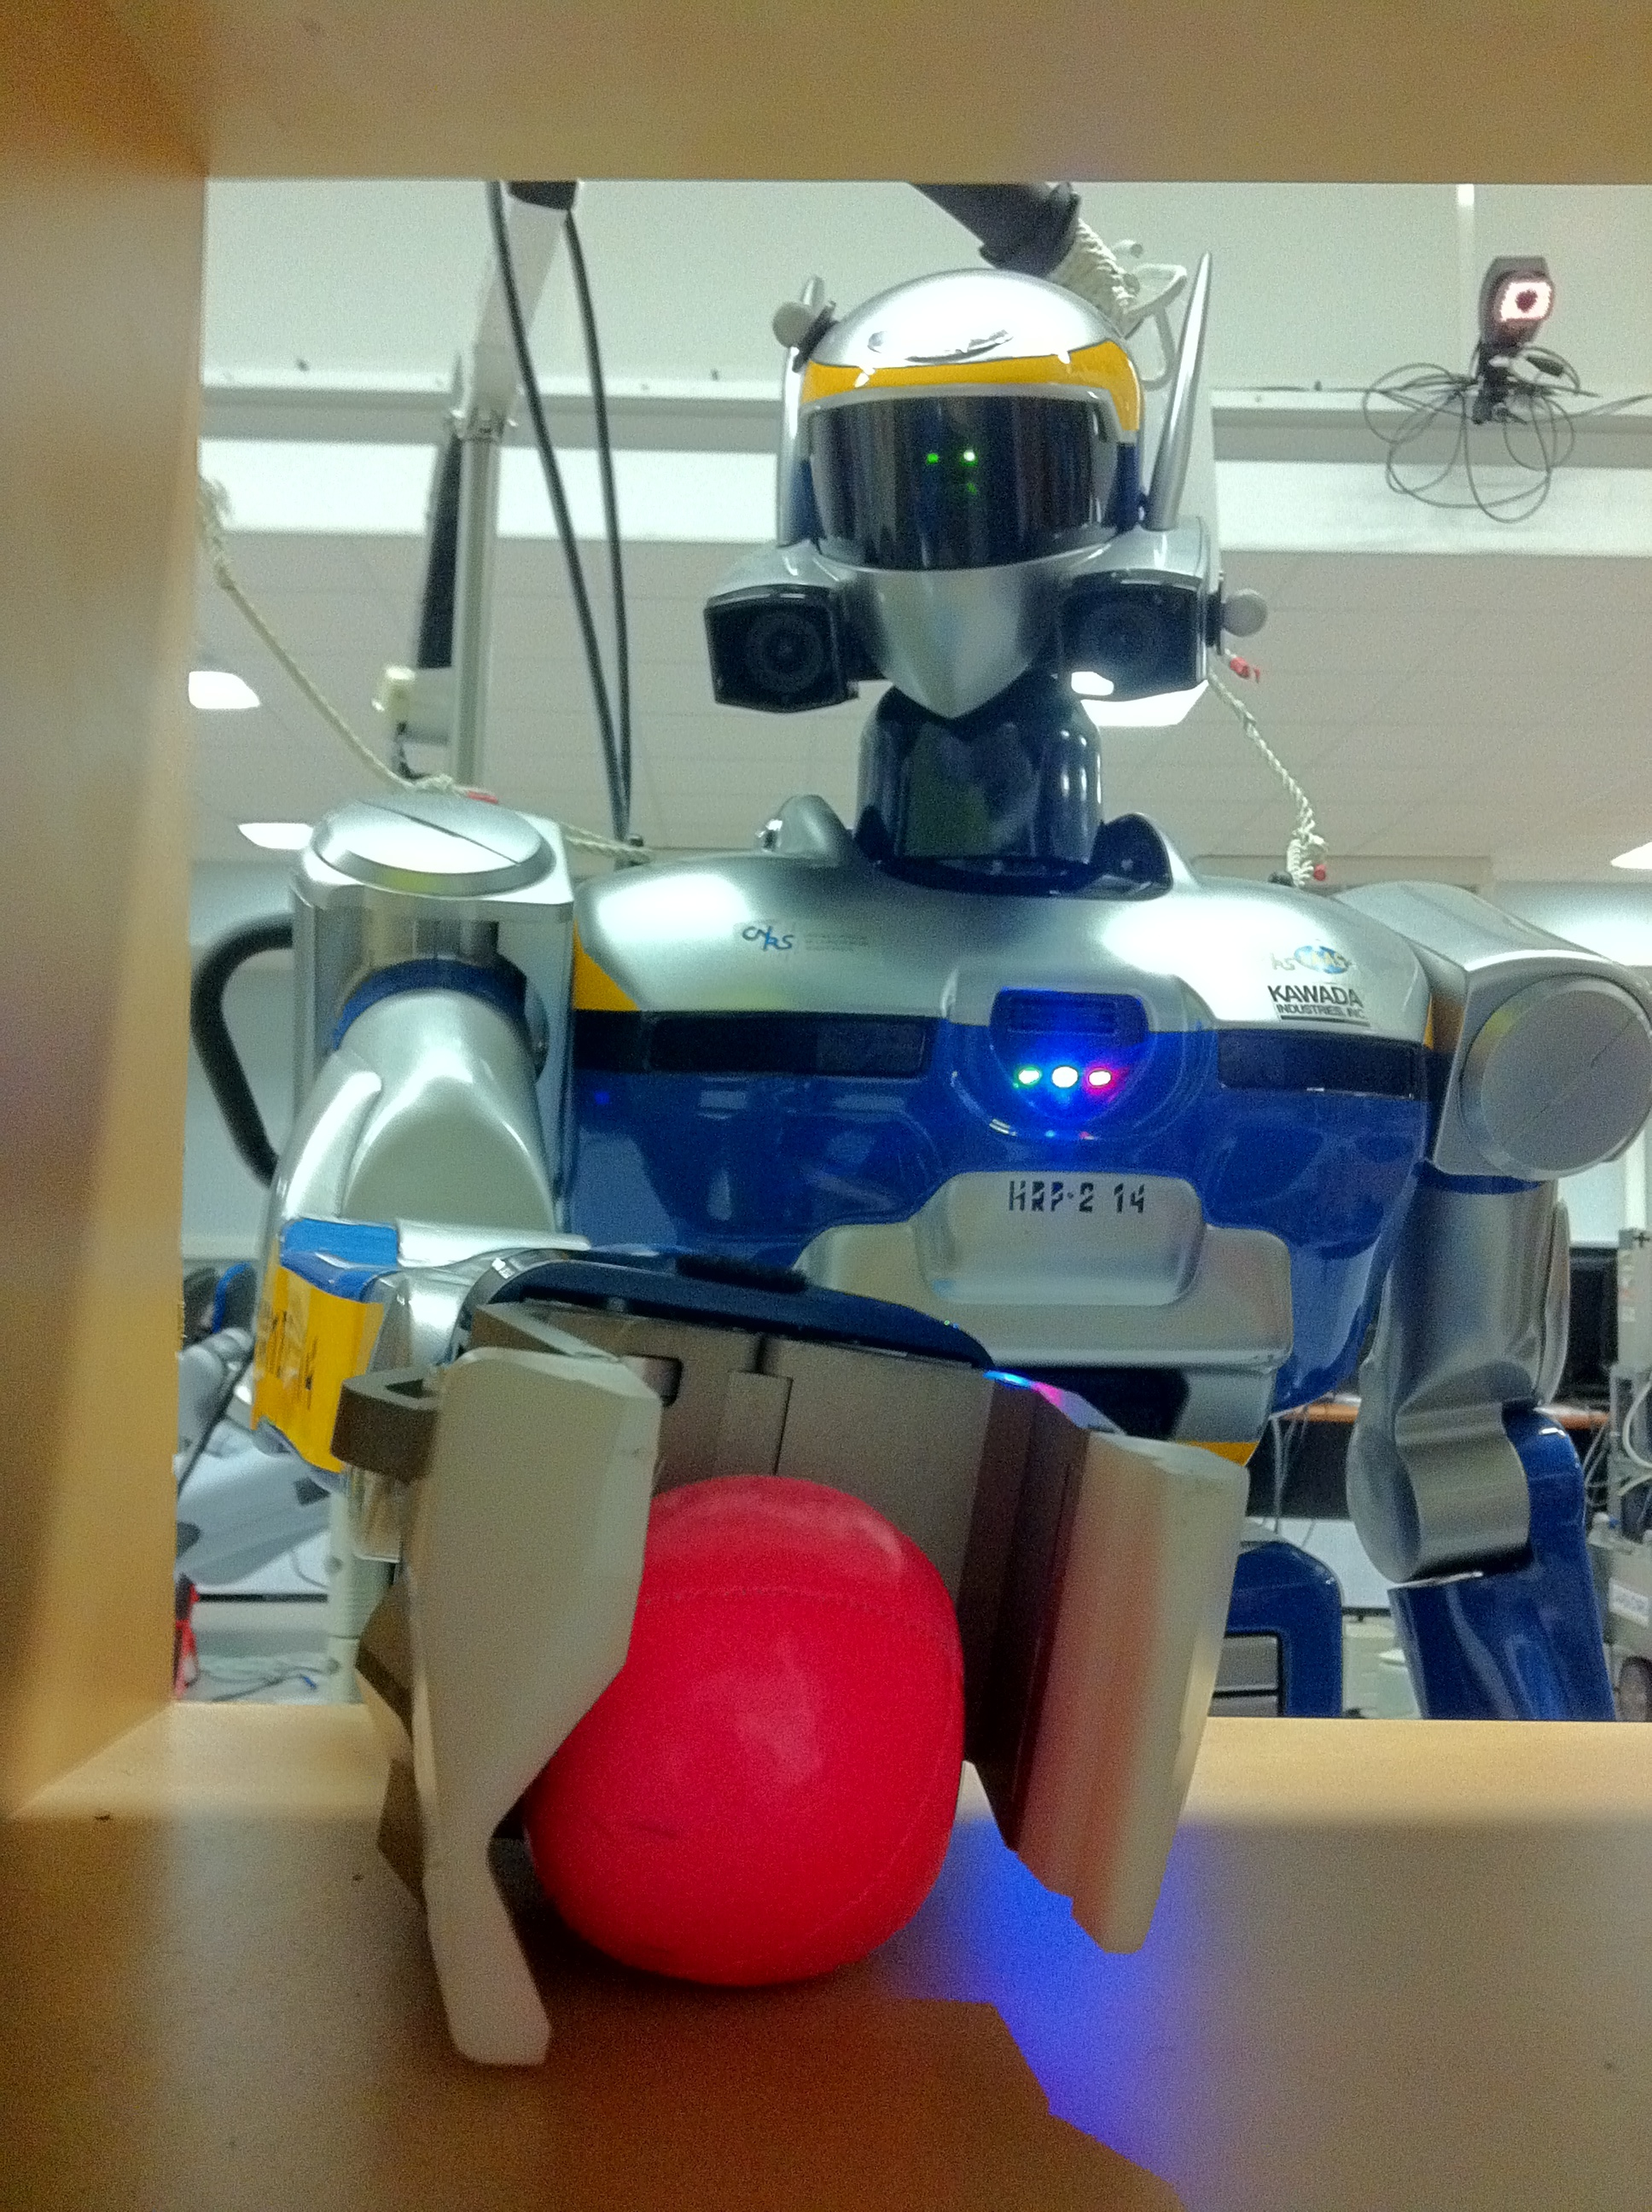
\includegraphics[width=\paperwidth,height=\paperheight]{%
      src/slides/demo1.jpg}}
  \begin{frame}[plain]
    \titlepage
  \end{frame}
}

%\maxFrameImage{src/slides/demo1.jpg}
%\maxFrameImage{src/slides/demo2.jpg}

% Introduction
% Animated scheme introducing contributions.
\begin{frame}
  \begin{changemargin}{-1cm}{-1cm}
    \begin{center}
      \tikzstyle{normalPath} = [line width=.7mm, color=black!50, -latex]

      \begin{tikzpicture}[
          auto,
          state/.style={
            rectangle,
            minimum size=6mm
          }]

        \uncover<1->{
          \node (perception) [state] {%
            
\includegraphics[height=3cm]{%
              src/slides/perception.pdf}};
        }

        \uncover<1>{
          \node (perception-description)
                [state, right=of perception]
                {\textbf{Perception}};
        }


        \uncover<2->{
          \node (decision)
               [state,above right=of perception] {%
            
\includegraphics[height=3cm]{%
              src/slides/decision.pdf}};
        }

        \uncover<2>{
          \node (decision-description)
                [state, right=of decision]
                {\textbf{Décision}};
        }

        \uncover<3->{
        \node (action) [state,below right=of decision]{%
          
\includegraphics[height=3cm]{%
            src/slides/action.pdf}};
        }

        \uncover<3>{
          \node (action-description)
                [state, left=of action]
                {\textbf{Action}};
        }

        \uncover<4->{
          \path (perception) edge[->, normalPath] (decision);
        }

        \uncover<5-8>{
          \path (decision) edge[->, normalPath] (action);
        }

        \uncover<6->{
          \path (action.south)
          edge[->, normalPath, dashed, bend right, bend left]
          node[color=black!50,above=5pt] {Monde réel}
          (perception.south);
        }

        \uncover<7->{
          \node (contrib) [state,left=of decision]{%
            \usebeamerfont{section}\large\textbf{Contributions}};

          \node (contrib1b) [state,right=1pt of decision]{%
            (1) RobOptim};
        }
        \uncover<7>{
          \node[thick,draw=ThoughfulBrick] (contrib1)
               [state,above=-3.4cm of decision] {%
                 \phantom{
\includegraphics[height=3.5cm]{%
                     src/slides/perception.pdf}}};
        }

        \uncover<8->{
          \path (perception.east)
          edge[->, normalPath,color=ThoughfulBrick]
          node[above=5pt] {(2) Correction}
          (action.west);
        }
        \uncover<8>{
          \node[thick,draw=ThoughfulBrick] (contrib2)
               [state,above=-3.4cm of action] {%
                 \phantom{
\includegraphics[height=3.5cm]{%
                     src/slides/action.pdf}}};
        }


        \uncover<9->{
          \path (decision) edge[->, normalPath,color=ThoughfulBrick]
          node[color=ThoughfulBrick,text width=3.5cm]{%
            (3) Primitives de mouvement} (action);
        }

        \uncover<10->{
          \node (contrib4b) [state,above=10pt of perception]{%
            (4) Intégration};
        }
        \uncover<10>{
          \node[thick,draw=ThoughfulBrick] (contrib4)
               [state,above=-3.4cm of perception] {%
                 \phantom{
\includegraphics[height=3.5cm]{%
                     src/slides/perception.jpg}}};
        }


      \end{tikzpicture}
    \end{center}
  \end{changemargin}
\end{frame}

\begin{slideDecision}
  \begin{changeleftmargin}{1.1cm}
    \frametitle{Processus de décision}
    \begin{center}
      \includegraphics%
          [width=.75\linewidth]%
          {src/chap1-roboptim/hrp2-two-chairs.png}

          \begin{enumerate}
          \item Planification.
          \item Optimisation de la trajectoire trouvée.
          \end{enumerate}
    \end{center}
  \end{changeleftmargin}
\end{slideDecision}

\begin{slideDecision}
  \begin{changeleftmargin}{1.1cm}
    \frametitle{Optimisation}
    \begin{equation*}
      \min_{\mathbf{x} \in \mathbb{R}^n} f(\mathbf{x})%
      \text{ sous la contrainte } \mathbf{x} \in \mathbf{X}
    \end{equation*}

    \begin{equation*}
      \mathbf{X} \equiv \left\{
      \begin{array}{l l}
        c_i (x) = 0    & \quad i \in \xi \\
        c_j (x) \leq 0 & \quad j \in \nu \\
      \end{array} \right.
    \end{equation*}

  \end{changeleftmargin}
\end{slideDecision}

\begin{slideDecision}
  \begin{changeleftmargin}{1.1cm}
    \frametitle{$\lambda$-calcul (1)}

    \begin{description}
      \item[Variables libres] $x$, $y$, \ldots
      \item[Application] $u v$ avec $u, v$ deux lambda-termes
      \item[Abstraction] $\lambda f x . t$ avec $x$ une variable, $t$
        un $\lambda$-terme.
    \end{description}
  \end{changeleftmargin}
\end{slideDecision}

\begin{slideDecision}
  \begin{changeleftmargin}{1.1cm}
    \frametitle{$\lambda$-calcul (2)}
    \begin{description}
      \item[Identité]~\\
        $\text{Id} \equiv \lambda x . x$
      \item[Entiers de Church]~\\
        $0 \equiv \lambda f x . x$\\
        $1 \equiv \lambda f x . f x$
      \item[Addition]~\\
        $\text{succ} \equiv \lambda n f x . f (n f x)$
    \end{description}
  \end{changeleftmargin}
\end{slideDecision}

\begin{slideDecision}
  \begin{changeleftmargin}{1.1cm}
    \frametitle{$\beta$-conversion}

    \begin{equation*}
      \begin{array}{ll}
      \text{succ}~1 & \rightarrow_\beta \lambda f x . (\lambda n f x . f (n f x)) (\lambda f x . f x)\\
        & \rightarrow_\beta \lambda f x . f ((\lambda f x . f x) f x)\\
        & \rightarrow_\beta \lambda f x . f f x \equiv 2\\
      \end{array}
    \end{equation*}

    \begin{center}
      \alert{réécrire $\equiv$ calculer $\equiv$ exécuter}
    \end{center}

  \end{changeleftmargin}
\end{slideDecision}

\begin{slideDecision}
  \begin{changeleftmargin}{1.1cm}
    \frametitle{$\lambda$-calcul simpement typé (1)}

    \begin{equation*}
      \Omega \equiv (\lambda x . x) (\lambda x . x)
    \end{equation*}

    \begin{equation*}
      (\lambda x . x) (\lambda x . x) =_\beta (\lambda x . x) (\lambda x . x)
    \end{equation*}
  \end{changeleftmargin}
\end{slideDecision}

\begin{slideDecision}
  \begin{changeleftmargin}{1.1cm}
    \frametitle{$\lambda$-calcul simpement typé (2)}

    \begin{description}
    \item[Type naturel]~\\
      $x \vdash \iota$
    \item[Type fonctionnel]~\\
      $x \vdash \iota \wedge t \vdash \tau \Rightarrow \lambda x. t \vdash \iota \rightarrow \tau$
    \end{description}

    \bigskip

    $\Omega$ n'est pas correctement typé.

  \end{changeleftmargin}
\end{slideDecision}

\begin{slideDecision}
  \begin{changeleftmargin}{1.1cm}
    \frametitle{Programmation orientée objet (1)}

    \begin{equation*}
      A \equiv \{ \underbrace{\{ \text{foo} \vdash \iota
        \}}_{\mathfrak{A}}, \underbrace{\{ \text{bar} \vdash A
        \rightarrow \iota, \text{baz} \vdash A \rightarrow \iota
        \}}_{\mathfrak{M}} \}
    \end{equation*}

    \begin{equation*}
      a \vdash A \Rightarrow a.\text{foo} \vdash \iota
    \end{equation*}

    \begin{equation*}
      a \vdash A \Rightarrow a.\text{bar} \vdash A \rightarrow \iota
    \end{equation*}
  \end{changeleftmargin}
\end{slideDecision}

\begin{slideDecision}
  \begin{changeleftmargin}{1.1cm}
    \frametitle{Programmation orientée objet (2)}

    \begin{equation*}
      u v \text{bien formé} \Rightarrow u \vdash \tau_1 \rightarrow
      \tau_2 \wedge \tau_3 <: \tau_1
    \end{equation*}

    \begin{equation*}
      \tau_2 <: \tau_1 \Rightarrow
      \mathfrak{A_{\tau_1}} \subset \mathfrak{A_{\tau_2}} \wedge \mathfrak{M_{\tau_1}} \subset
      \mathfrak{M_{\tau_2}}
    \end{equation*}
  \end{changeleftmargin}
\end{slideDecision}

\begin{slideDecision}
  \begin{changeleftmargin}{1.1cm}
    \frametitle{Type paramétré}

    Fonction d'ordre supérieur $\text{type}
    \Rightarrow \text{type}$.

    \bigskip

    Exemple: $\tau_\alpha$
  \end{changeleftmargin}
\end{slideDecision}

\begin{slideDecision}
  \begin{changeleftmargin}{1.1cm}
    \frametitle{Représentation du problème (1)}

    \begin{equation*}
      \text{Fonction} \equiv \{ \underbrace{\{ \#\text{entrée} \vdash
        \iota \}}_{\text{attributs}}, \underbrace{\{ \text{calcule}
        \vdash \text{Fonction} \rightarrow[\iota] \rightarrow \iota \}}_{\text{méthode}} \}
    \end{equation*}

    \begin{equation*}
      \text{FonctionDérivable} \equiv \{ \{ \}, \{ \text{gradient}
      \vdash \text{FonctionDérivable} \rightarrow [\iota] \rightarrow [\iota] \} \} <: \text{Fonction}
    \end{equation*}

  \end{changeleftmargin}
\end{slideDecision}

\begin{slideDecision}
  \begin{changeleftmargin}{1.1cm}
    \frametitle{Représentation du problème (2)}

  \begin{equation*}
  \begin{split}
    \text{Fonction}_n \equiv
    \left\{
    \begin{array}{l l}
      \text{Fonction} & \quad \text{si $n = 0$}\\
      \text{FonctionDérivable} & \quad \text{si $n = 1$}\\
      \{ \{ \}, \{ \text{gradient} \vdash \text{Fonction}_n \rightarrow \iota \rightarrow [\iota] \rightarrow [\iota] \} \} <: \text{Fonction}_{n-1} & \quad \text{si $n > 1$}\\
    \end{array} \right.
  \end{split}
  \end{equation*}

  \end{changeleftmargin}
\end{slideDecision}

\begin{slideDecision}
  \begin{changeleftmargin}{1.1cm}
    \frametitle{Représentation du problème (3)}

  \begin{equation*}
  \begin{split}
    \tau_{\text{prob}(\tau_1, \tau_2, \tau_3, \dotsc)} \equiv
    \{ \{ & \text{coût} \vdash \tau_1,\\
    & \text{contraintes} \vdash [\cup_{i \in \{2, \dotsc, n\}} \tau_i],\\
    & \text{bornes\_contraintes\_min} \vdash [\iota], \\
    & \text{bornes\_contraintes\_max} \vdash [\iota] \},\\
    & \{ \} \}\\
  \end{split}
  \end{equation*}

  \begin{equation*}
    \text{Solveur}_{\tau} \equiv \{ \{ \}, \{ \text{résous} \vdash
    \text{Solveur}_{\tau} \rightarrow \tau \rightarrow [\iota] \} \}
  \end{equation*}
  \end{changeleftmargin}
\end{slideDecision}

\begin{slideDecision}
  \begin{changeleftmargin}{1.1cm}
    \frametitle{Exemple: Optimisation non linéaire}

    \begin{description}
    \item[Fonction de coût]~\\
      $\text{Fonction}_2$
    \item[Contraintes linéaires]~\\
      $\text{FonctionLinéaire}$
    \item[Contraintes non linéaires]~\\
      $\text{Fonction}_2$
    \item[Problème]
    \end{description}

    ~~~~$\text{Problème}_{\text{prob}(\text{Fonction}_2, \text{FonctionLinéaire}, \text{Fonction}_2)}$

  \end{changeleftmargin}
\end{slideDecision}


\begin{slideDecision}
  \frametitle{RobOptim}
\end{slideDecision}

\begin{slideDecision}
  \frametitle{Applications}
\end{slideDecision}


\begin{slideAction}
  \frametitle{La marche bipède (1)}

  \begin{equation*}
    \begin{array}{lll}
    x_{ZMP} &=& x_G - \frac{\dot{\sigma}_y\ +\ m\ z_G\ \ddot{x}_G}{m\ (\ddot{z}_G + g)}\\
    y_{ZMP} &=& y_G + \frac{\dot{\sigma}_x\ -\ m\ z_G\ \ddot{y}_G}{m\ (\ddot{z}_G + g)}
    \end{array}
  \end{equation*}
\end{slideAction}

\maxFrameImageHeight{src/chap3-primitive-mouvement/footsteps1.jpg}
\maxFrameImageHeight{src/chap3-primitive-mouvement/calibextrinsic.jpg}

\begin{slideAction}
  \frametitle{Contrôleur polyvalent pour la robotique}

  \begin{equation*}
    \mathbf{e} = \mathbf{s} - \mathbf{s}^{*}
  \end{equation*}
  
  \begin{equation*}
    \mathbf{J}_i = \frac{\partial \mathbf{e}_i}{\partial \mathbf{q}}
  \end{equation*}

  \begin{equation*}
    \dot{\mathbf{e}}_i = \mathbf{J}_i \dot{\mathbf{q}}
  \end{equation*}

  \begin{equation*}
    \dot{\mathbf{q}} = \mathbf{J}_1^{+} \dot{\mathbf{e}}_1^{*} + \mathbf{P}_1 \mathbf{z}
  \end{equation*}

  \begin{equation*}
    \mathbf{P}_1 = \mathbf{I} - \mathbf{J}_1^{+} \mathbf{J}_1
  \end{equation*}

  \begin{equation*}
    \mathbf{z} = \mathbf{J}_2^{+} \dot{\mathbf{e}}_2^{*}
  \end{equation*}

  \begin{equation*}
    \mathbf{s}_1^{*} = -\lambda (\mathbf{s}_1 - \mathbf{s}_1{*})
  \end{equation*}

\end{slideAction}




\begin{slideAction}
  \frametitle{Schéma de contrôle boucle fermée}

  FIXME
\end{slideAction}

\maxFrameImageHeight{src/chap2-suivi-trajectoire/demo.jpg}

\begin{slideAction}
  \frametitle{Correction de la pile de pas}

  FIXME
\end{slideAction}

\begin{slideAction}
  \frametitle{Correction de la trajectoire des pieds}

  FIXME
\end{slideAction}

\begin{slideAction}
  \frametitle{Correction de la trajectoire du centre de masse}

  FIXME
\end{slideAction}


\begin{slideAction}
  \frametitle{Résultats expérimentaux}

  FIXME
\end{slideAction}


\begin{slidePerception}
  \frametitle{Du magnétophone au robot}

  FIXME
\end{slidePerception}

\begin{slidePerception}
  \frametitle{De la bibliothèque au composant}

  FIXME
\end{slidePerception}

\maxFrameImageHeight{src/slides/demo2.jpg}

\maxFrameImageHeight{src/chap4-integration/footsteps2.jpg}
\maxFrameImageHeight{src/chap4-integration/disparity-1.jpg}
\maxFrameImageHeight{src/chap4-integration/disparity-2.jpg}
\maxFrameImageHeight{src/chap4-integration/hrp2_urdf.jpg}
\maxFrameImageHeight{src/chap4-integration/rviz-full.jpg}
\maxFrameImageHeight{src/chap4-integration/shelf.png}

\begin{slidePerception}
  \frametitle{Résultats}
  FIXME
\end{slidePerception}


\begin{frame}
  CONCLUSION
\end{frame}

\maxFrameImageHeight{src/slides/hrp2-thx.jpg}


\end{document}
